\chapter{Operaciones de Modelado}

\begin{figure}[H]
	\centering
	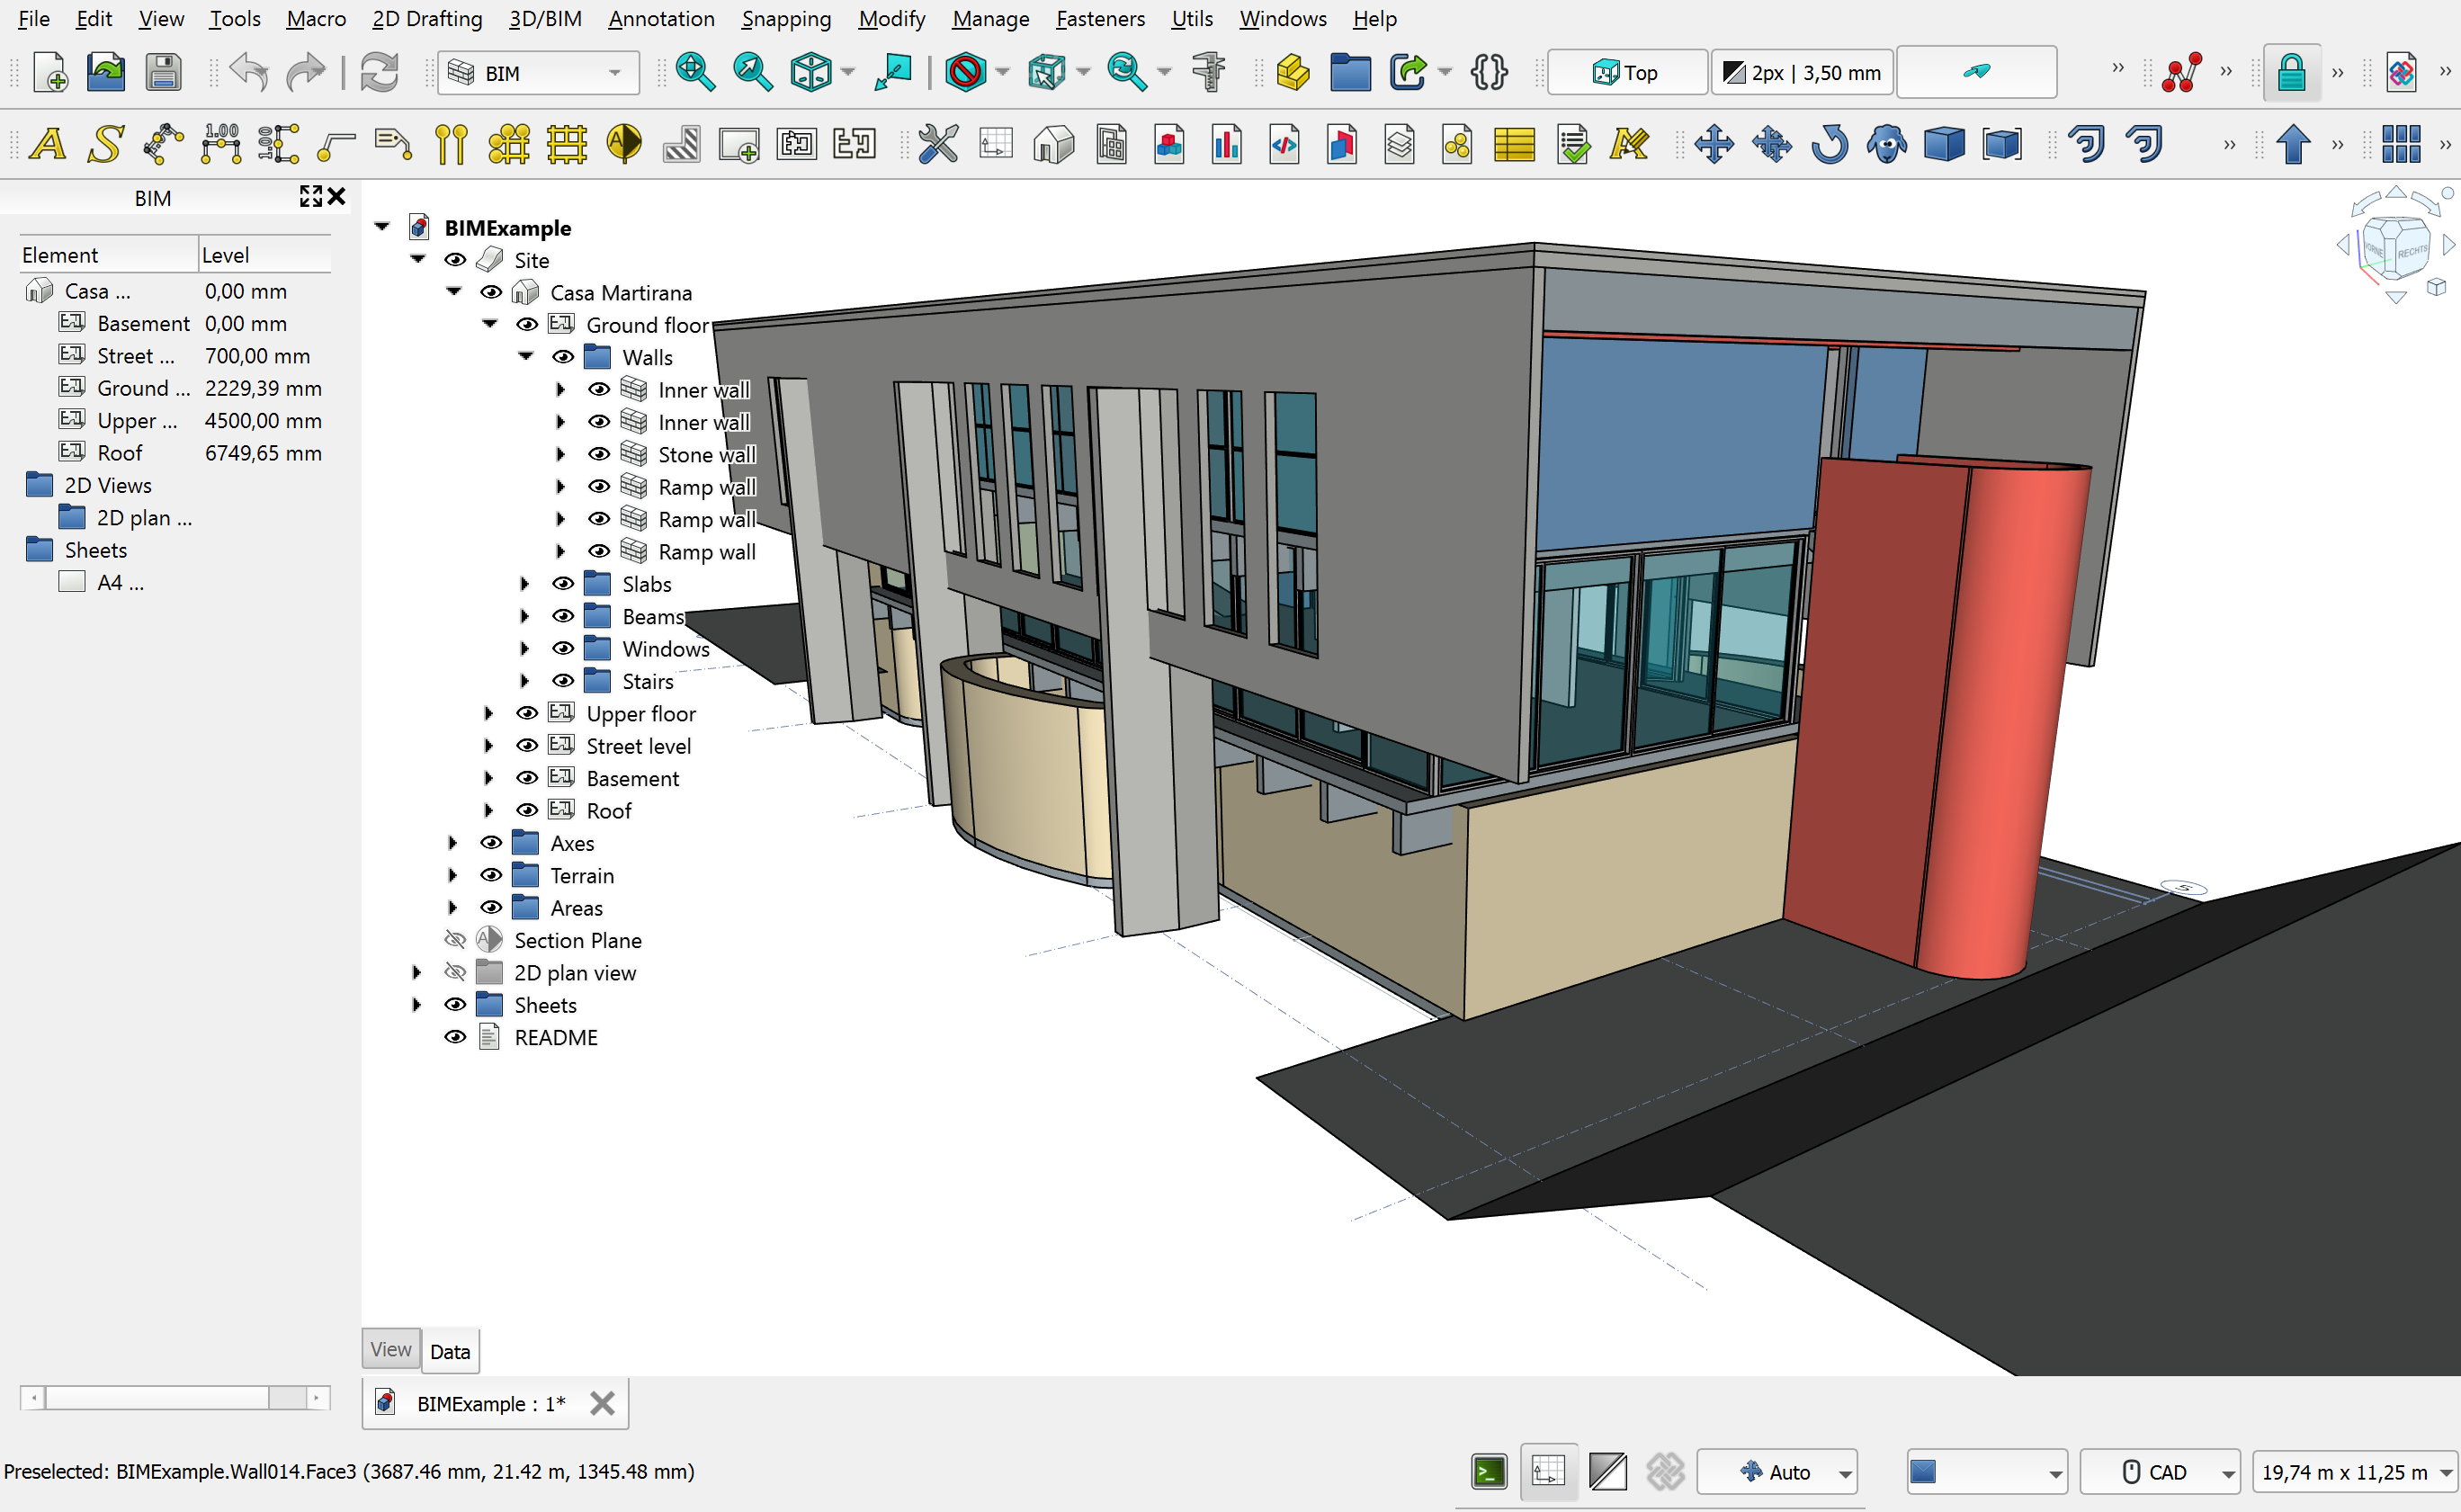
\includegraphics[width=0.8\textwidth]{img/cap6_operaciones.png}
	\caption{Modelo 3D creado con operaciones de extrusión y revolución}
\end{figure}

Aprende las operaciones fundamentales de modelado 3D:
extrusión, revolución y loft. Convierte bocetos 2D
en sólidos complejos.

%% D. Búsqueda e Inserción de Activos Gráficos
%% Imagen insertada al inicio del capítulo

%% B. Actividades Teóricas
\section{Investigar y responder}
\faPencil

Investiga sobre operaciones de modelado y responde:
\begin{enumerate}
	\item ¿Qué es la operación de extrusión (pad) y cómo
	      se aplica?
	\item ¿Cómo funciona la operación de revolución (revolve)?
	\item ¿Qué es la operación de loft y cuándo se utiliza?
	\item ¿Cómo se crean agujeros (pockets) en sólidos?
	\item ¿Qué es el biselado (fillet) y el chaflanado
	      (chamfer)?
	\item ¿Cómo se combinan múltiples operaciones en un
	      modelo?
	\item ¿Qué significa ``historial de operaciones'' en
	      FreeCAD?
	\item ¿Cómo se modifican operaciones después de creadas?
\end{enumerate}

%% C. Actividades Prácticas
\section{Resolver los siguientes problemas}
\faWrench

Problemas para aplicar conocimientos:
\begin{enumerate}
	\item Crea un prisma rectangular extrusionando un
	      rectángulo de 100x50 mm a 30 mm de altura.
	\item Modela un cilindro hueco usando la operación
	      de revolución.
	\item Crea una pieza con múltiples extrusiones de
	      diferentes alturas.
	\item Modela una pieza con agujero cilíndrico pasante.
	\item Practica el biselado de aristas con diferentes
	      radios.
	\item Crea un chaflán de 45 grados en las aristas
	      de un cubo.
	\item Modela una pieza simple de una hélice usando
	      operación de loft.
	\item Crea una pieza que combine extrusión y
	      revolución.
	\item Modifica la altura de una extrusión en un modelo
	      existente.
	\item Modela una pieza mecánica simple como un soporte
	      con varias operaciones.
\end{enumerate}